\begin{frame}[allowframebreaks]{Method 1: Shamir Threshold SSS \cite{shamir1979}}
	\textbf{\textcolor{blue}{Access structure: \(t\)-out-of-\(n\)}}
	\[
	\mathcal{A}_t = \{A\subseteq \mathcal{P}\;:\;|A|\ge t\}.
	\]

	\textbf{\textcolor{blue}{Sharing idea}}
	\begin{itemize}
		\item Work over a finite field \(\mathbb{F}_q\) (prime power), choose distinct nonzero points \(x_1,\dots,x_n\in\mathbb{F}_q\).
		\item Sample random coefficients \(\alpha_1,\dots,\alpha_{t-1}\leftarrow \mathbb{F}_q\).
		\item Define degree-\((t-1)\) polynomial:
		\[
		P(x) = s + \alpha_1x + \cdots + \alpha_{t-1}x^{t-1}.
		\]
		\item Give share \((x_i,\,P(x_i))\) to party \(P_i\).
	\end{itemize}

	\textbf{\textcolor{blue}{Why it works}}
	\begin{itemize}
		\item Any \(t\) points interpolate a degree-\((t-1)\) polynomial \(\Rightarrow\) reconstruct \(s=P(0)\).
		\item Any \(t-1\) shares reveal no information about \(s\) (perfect privacy).
		\item Threshold schemes are often used as the baseline due to simplicity and efficiency.
	\end{itemize}

	\begin{figure}
		\centering
		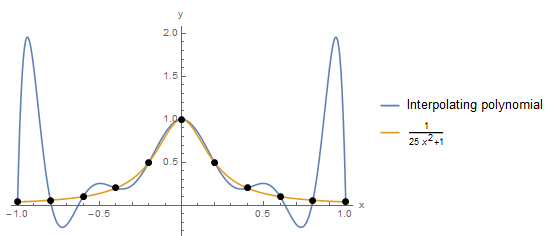
\includegraphics[scale=0.5]{fig/fig-lagrange-interpolation.png}
		\caption{Lagrange Interpolation of \(f(x) = \frac{1}{25x^2 + 1}\)}
	\end{figure}
\end{frame}

\begin{frame}{Reconstruction (Lagrange Interpolation)}
	Given any authorized set \(A=\{i_1,\dots,i_t\}\) with shares \((x_{i_j}, y_{i_j})\) where \(y_{i_j}=P(x_{i_j})\),
	\[
	s = P(0) = \sum_{j=1}^{t} y_{i_j}\cdot \lambda_{i_j}(0),
	\quad
	\lambda_{i_j}(0)=\prod_{\ell\neq j}\frac{0-x_{i_\ell}}{x_{i_j}-x_{i_\ell}}
	\quad \text{in } \mathbb{F}_q.
	\]

	{\scriptsize
	\SetAlCapFnt{\scriptsize}
	\SetAlCapNameFnt{\scriptsize}
	\begin{algorithm}[H]
		\caption{Shamir-Reconstruct(\(t\) shares)}
		\DontPrintSemicolon
		\KwInput{\(t\) pairs \((x_1,y_1),\dots,(x_t,y_t)\) in \(\mathbb{F}_q^2\)}
		\KwOutput{Secret \(s=P(0)\)}
		\BlankLine
		Compute \(c_j \leftarrow \prod_{\ell\neq j}\dfrac{-x_\ell}{x_j-x_\ell}\) for each \(j\in\{1,\dots,t\}\)\;
		Return \(s \leftarrow \sum_{j=1}^{t} y_j \cdot c_j\)\;
	\end{algorithm}
	}

	\textbf{\textcolor{blue}{Note}}: implementations often precompute coefficients for fixed \(x_i\).
\end{frame}
